\documentclass{bioinfo}
\copyrightyear{2005}
\pubyear{2005}

\begin{document}
\firstpage{1}

\title[short Title]{roche454QAreport an ``R" package for Roche 454 Pyrosequencing Quality Assurance}
\author[Sample \textit{et~al}]{Matt L. Settles\,$^{1}$ and Zev N. Kronenberg \,$^{1}$\footnote{Corresponding author: Matt L. Settles, mattsettles@gmail.com}}
\address{$^{1}$Department of Biological Sciences, University of Idaho, Room 252, Life Sciences South, University of Idaho, PO Box 443051 Moscow, ID 83844-3051 USA.}

\history{Received on XXXXX; revised on XXXXX; accepted on XXXXX}

\editor{Associate Editor: XXXXXXX}

\maketitle

\begin{abstract}

\section{Motivation:}

Quality metrics associated with Roche 454 pyrosequencing runs are spread across several files. 
Without an advanced understanding of file contents and what each quality metric means, it may be difficult for researchers to understand how successful their sequencing project was.
It is the Roche technician's job to covey informative data regarding the success of a 454 to these end users.  
Until now there wasn't a software package, openly available, to automatically generate a quality assurance report.
The aim of our software package was to provide a quality assurance report so that Roche technicians, can rapidly check the quality of the run and share that information with researchers. 


\section{Results:}
The output of this software package is a multi-page PDF document that contain graphs, tables, and explanations of quality metrics for a 454 run. 

\section{Availability:}
This package and source code is available at Bioconductor 
\section{Contact: mattsettles@gmail.com} \href{http://bioinfo-mite.ibest.uidaho.edu/}
\end{abstract}

\section{Introduction}
%Figure~ \ref{fig:01} shows that the above method
A Roche 454 sequences produces large images of 
This program produces a data directory that is populated by files that contain sequence data as well as quality information.
The *.fna files contain FASTA formated DNA sequence data and the *.qual files contain FASTQ formatted PHRED quality scores (\citealp{Cock2010}).
A PHRED quality score is a transformed estimated probability of a DNA base being incorrectly called (\citealp{Ewing1998a,Ewing1998b}). 
Equation~\ref{eq:01} describes the log transformed (q) estimated error probability (p) for any particular DNA base in a FASTA sequence.       
  
\begin{equation}
q = -10*\log_10(p)  \label{eq:01}
\end{equation}



\begin{methods}
\section{Methods}

Text Text Text Text Text Text  Text Text Text Text Text Text Text Text Text  Text Text Text Text Text Text. Figure \ref{fig:02} shows that the above method  Text Text Text Text  Text Text Text Text Text Text  Text Text.  \citealp{shortread} might want to know about  text text text text
Text Text Text Text Text Text  Text Text Text Text Text Text Text Text Text  Text Text Text Text Text Text. Figure \ref{fig:02} shows that the above method  Text Text Text Text  Text Text Text Text Text Text  Text Text.  \citealp{shortread} might want to know about  text text text text
Text Text Text Text Text Text  Text Text Text Text Text Text Text Text Text  Text Text Text Text Text Text. Figure \ref{fig:02} shows that the above method  Text Text Text Text  Text Text Text Text Text Text  Text Text.  \citealp{shortread} might want to know about  text text text text

\begin{itemize}
\item for bulleted list, use itemize
\item for bulleted list, use itemize
\item for bulleted list, use itemize
\end{itemize}



Text Text Text Text Text Text  Text Text Text Text Text Text Text Text Text  Text Text Text Text Text Text. Figure \ref{fig:02} shows that the above method  Text Text Text Text  Text Text Text Text Text Text  Text Text.  \citealp{shortread} might want to know about  text text text text
Text Text Text Text Text Text  Text Text Text Text Text Text Text Text Text  Text Text Text Text Text Text. Figure \ref{fig:02} shows that the above method  Text Text Text Text  Text Text Text Text Text Text  Text Text.  \citealp{shortread} might want to know about  text text text text
Text Text Text Text Text Text  Text Text Text Text Text Text Text Text Text  Text Text Text Text Text Text. Figure \ref{fig:02} shows that the above method  Text Text Text Text  Text Text Text Text Text Text  Text Text.  \citealp{shortread} might want to know about  text text text text
Text Text Text Text Text Text  Text Text Text Text Text Text Text Text Text  Text Text Text Text Text Text. Figure \ref{fig:02} shows that the above method  Text Text Text Text  Text Text Text Text Text Text  Text Text.  \citealp{shortread} might want to know about  text text text text
Text Text Text Text Text Text  Text Text Text Text Text Text Text Text Text  Text Text Text Text Text Text.


Text Text Text Text Text Text  Text Text Text Text Text Text Text Text Text  Text Text Text Text Text Text. Figure \ref{fig:02} shows that the above method  Text Text Text Text  Text Text Text Text Text Text  Text Text.  \citealp{shortread} might want to know about  text text text text
Text Text Text Text Text Text  Text Text Text Text Text Text Text Text Text  Text Text Text Text Text Text. Figure \ref{fig:02} shows that the above method  Text Text Text Text  Text Text Text Text Text Text  Text Text.  \citealp{shortread} might want to know about  text text text text
Text Text Text Text Text Text  Text Text Text Text Text Text Text Text Text  Text Text Text Text Text Text. Figure \ref{fig:02} shows that the above method  Text Text Text Text  Text Text Text Text Text Text  Text Text.  \citealp{shortread} might want to know about  text text text text



Text Text Text Text Text Text  Text Text Text Text Text Text Text Text Text  Text Text Text Text Text Text. Figure \ref{fig:02} shows that the above method  Text Text Text Text  Text Text Text Text Text Text  Text Text.  \citealp{shortread} might want to know about  text text text text
Text Text Text Text Text Text  Text Text Text Text Text Text Text Text Text  Text Text Text Text Text Text. Figure \ref{fig:02} shows that the above method  Text Text Text Text  Text Text Text Text Text Text  Text Text.  \citealp{shortread} might want to know about  text text text text
Text Text Text Text Text Text  Text Text Text Text Text Text Text Text Text  Text Text Text Text Text Text. Figure \ref{fig:02} shows that the above method  Text Text Text Text  Text Text Text Text Text Text  Text Text.  \citealp{shortread} might want to know about  text text text text


Text Text Text Text Text Text  Text Text Text Text Text Text Text Text Text  Text Text Text Text Text Text. Figure \ref{fig:02} shows that the above method  Text Text Text Text  Text Text Text Text Text Text  Text Text.  \citealp{shortread} might want to know about  text text text text
Text Text Text Text Text Text  Text Text Text Text Text Text Text Text Text  Text Text Text Text Text Text. Figure \ref{fig:02} shows that the above method  Text Text Text Text  Text Text Text Text Text Text  Text Text.  \citealp{shortread} might want to know about  text text text text
Text Text Text Text Text Text  Text Text Text Text Text Text Text Text Text  Text Text Text Text Text Text. Figure \ref{fig:02} shows that the above method  Text Text Text Text  Text Text Text Text Text Text  Text Text.  \citealp{shortread} might want to know about  text text text text



\begin{table}[!t]
\processtable{Summary of quality filter metrics extracted from ``454QualityFilterMetrics.csv.” Rows 5-10 are the values associated with the key sequences, and rows 12-17 are associated with the experimental sequences. This particular experiment had four regions as seen in columns 2:5. This table automatically scales the number of columns to match the number of regions.\label{Tab:01}}
{\begin{tabular}{llllll}
  \hline
 & region & 1 & 2 & 3 & 4 & \\ 
  \hline
 
  & totalRawWells & 309306 & 374784 & 228460 & 166751 \\ 
  & totalKeyPass & 304856 & 370609 & 223750 & 158656 \\ 
  & keySequence & CATG & CATG & CATG & CATG \\ 
  & numKeyPass & 3181 & 8527 & 6070 & 5207 \\ 
  & numDotFailed & 2 & 12 & 23 & 32 \\ 
  & numMixedFailed & 14 & 69 & 35 & 15 \\ 
  & numTrimmedTooShortQuality & 55 & 350 & 176 & 49 \\ 
  & numTrimmedTooShortPrimer & 0 & 0 & 0 & 0 \\ 
  & totalPassedFiltering & 3110 & 8096 & 5836 & 5111 \\ 
  & keySequence & TCAG & TCAG & TCAG & TCAG \\ 
  & numKeyPass & 301675 & 362082 & 217680 & 153449 \\ 
  & numDotFailed & 26731 & 19064 & 3149 & 3108 \\ 
  & numMixedFailed & 50075 & 13578 & 17921 & 3822 \\ 
  & numTrimmedTooShortQuality & 90767 & 101477 & 41645 & 21666 \\ 
  & numTrimmedTooShortPrimer & 0 & 0 & 0 & 0 \\ 
  & totalPassedFiltering & 134102 & 227963 & 154965 & 124853 \\ 
   \hline

\end{tabular}}{This is a footnote}
\end{table}

\end{methods}

\begin{figure}[!tpb]
\centerline{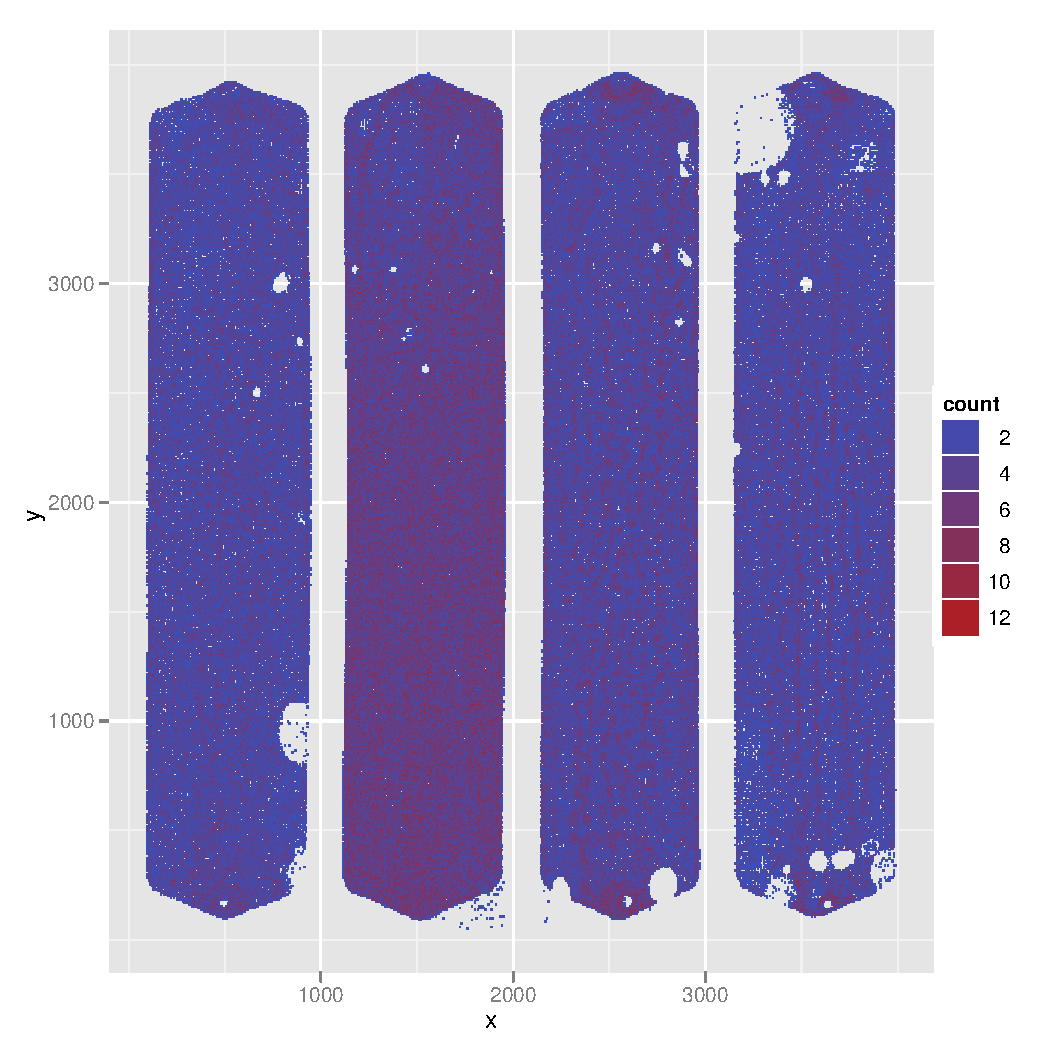
\includegraphics[width=9 cm]{heatmap.pdf}}
\caption{Heatmap illustrating the number of reads mapped to their physical locations on the plate. Regions 1:4 were drawn from left to right. This plot represents those reads that passed quality filtering.  Reads were grouped with the parameter: bin, which is part of the stat$\_$bin command in the ggplot2 package.  The second region had the greatest number of reads.  }
\end{figure}

\begin{figure}[!tpb]%figure2
%\centerline{\includegraphics{fig02.eps}}
\caption{Caption, caption.}\label{fig:02}
\end{figure}

}

\section{Discussion}

Text Text Text Text Text Text  Text Text Text Text Text Text Text Text Text  Text Text Text Text Text Text. Figure \ref{fig:02} shows that the above method  Text Text Text Text  Text Text Text Text Text Text  Text Text.  \citealp{shortread} might want to know about  text text text text
Text Text Text Text Text Text  Text Text Text Text Text Text Text Text Text  Text Text Text Text Text Text. Figure \ref{fig:02} shows that the above method  Text Text Text Text  Text Text Text Text Text Text  Text Text.  \citealp{shortread} might want to know about  text text text text
Text Text Text Text Text Text  Text Text Text Text.




Table~\ref{Tab:01} shows that Text Text Text Text Text  Text Text Text Text Text Text. Figure \ref{fig:02} shows that
the above method Text Text. Text Text Text  Text Text Text Text Text Text. Figure \ref{fig:02} shows that
the above method Text Text. Text Text Text  Text Text Text Text Text Text. Figure \ref{fig:02} shows that
the above method Text Text.









%%%%%%%%%%%%%%%%%%%%%%%%%%%%%%%%%%%%%%%%%%%%%%%%%%%%%%%%%%%%%%%%%%%%%%%%%%%%%%%%%%%%%
%
%     please remove the " % " symbol from \centerline{\includegraphics{fig01.eps}}
%     as it may ignore the figures.
%
%%%%%%%%%%%%%%%%%%%%%%%%%%%%%%%%%%%%%%%%%%%%%%%%%%%%%%%%%%%%%%%%%%%%%%%%%%%%%%%%%%%%%%






\section{Conclusion}

(Table~\ref{Tab:01}) Text Text Text Text Text Text  Text Text Text Text Text Text Text Text Text  Text Text Text Text Text Text. Figure \ref{fig:02} shows that the above method  Text Text Text Text  Text Text Text Text Text Text  Text Text.  \citealp{shortread} might want to know about  text text text text
Text Text Text Text Text Text  Text Text Text Text Text Text Text Text Text  Text Text Text Text Text Text. Figure \ref{fig:02} shows that the above method  Text Text Text Text  Text Text Text Text Text Text  Text Text.  \citealp{shortread} might want to know about  text text text text
Text Text Text Text Text Text  Text Text Text Text Text Text Text Text Text  Text Text Text Text Text Text. Figure \ref{fig:02} shows that the above method  Text Text Text Text  Text Text Text Text Text Text  Text Text.



Text Text Text Text Text Text  Text Text Text Text Text Text Text Text Text  Text Text Text Text Text Text. Figure \ref{fig:02} shows that the above method  Text Text Text Text  Text Text Text Text Text Text  Text Text.  \citealp{shortread} might want to know about  text text text text





\begin{enumerate}
\item this is item, use enumerate
\item this is item, use enumerate
\item this is item, use enumerate
\end{enumerate}

Text Text Text Text Text Text  Text Text Text Text Text Text Text Text Text  Text Text Text Text Text Text. Figure \ref{fig:02} shows that the above method  Text Text Text Text  Text Text Text Text Text Text  Text Text.  \citealp{shortread} might want to know about  text text text text
Text Text Text Text Text Text  Text Text Text Text Text Text Text Text Text  Text Text Text Text Text Text. Figure \ref{fig:02} shows that the above method  Text Text Text Text  Text Text Text Text Text Text  Text Text.  \citealp{shortread} might want to know about  text text text text
Text Text Text Text Text Text  Text Text Text Text Text Text Text Text Text  Text Text Text Text Text Text.






Text Text Text Text Text Text  Text Text Text Text Text Text Text Text Text  Text Text Text Text Text Text. Figure \ref{fig:02} shows that the above method  Text Text Text Text


\section*{Acknowledgement}
Text Text Text Text Text Text  Text Text.  \citealp{shortread} might want to know about  text text text text

\paragraph{Funding\textcolon} Text Text Text Text Text Text  Text Text.

%\bibliographystyle{natbib}
%\bibliographystyle{achemnat}
%\bibliographystyle{plainnat}
%\bibliographystyle{abbrv}
%\bibliographystyle{bioinformatics}
%
%\bibliographystyle{plain}
%
%\bibliography{Document}


\begin{thebibliography}{}
\bibliographystyle{natbib}
\bibliography{cite}
\end{thebibliography}
\end{document}
